 \chapter{Diseño} \label{sec:design}
    En este apartado se ofrece una descripción de las decisiones tomadas a nivel de diseño a lo largo del desarrollo de la aplicación web.
    
    \section{Arquitectura del Sistema}
    Desde un punto de vista lo suficientemente alejado como para no percibir los detalles internos, la aplicación web está organizada siguiendo la arquitectura clásica cliente-servidor-datos. Hoy en día, quizás, esta no sea la organización más vanguardista. Los términos \emph{serverless}, \emph{microservicios} o \emph{single-page-application} son los que con mayor eco resuenan en la industria web actual.
    
    \begin{figure}[h]
    	\centering
    	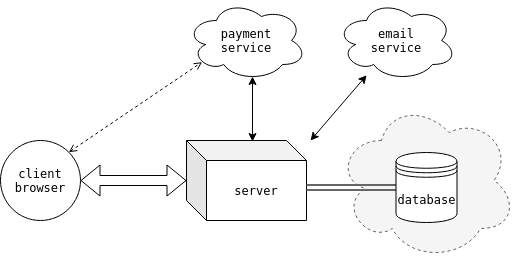
\includegraphics[width=\textwidth]{desing_general}
    	\caption{Modelo del sistema}
    	\label{fig:desing_general}
    \end{figure}
    
    Como muchas tendencias dentro del mundo de la computación, estos términos no están del todo delimitados, ofreciendo en ocasiones diferentes interpretaciones y/o solapamientos entre sí. Serverless hace mención a aquellas aplicaciones web que en su mayor parte, o por completo, incorporan servicios cloud de terceras partes para gestionar su propia lógica de negocio. La arquitectura de microservicios está muy relacionada con lo anterior, ya que esta concibe las aplicaciones como un agregado de servicios muy especializados ejecutados de forma independiente, puede que en máquinas remotas, que se comunican entre sí de manera ligera y eficiente. Por su parte, las SPA usan la elevada capacidad de cómputo de los clientes actuales para trasladar allí parte de la lógica que tradicionalmente implementa el servidor. En una SPA o bien todo el contenido HTML, JavaScript y CSS es cargado una sola vez, o bien se carga dinámicamente bajo demanda, normalmente como respuesta a las acciones del usuario, dando así una mayor sensación de fluidez.
    
    No obstante, a pesar de las muchas ventajas que presentan estas formas de enfocar las aplicaciones web, se ha optado por la arquitectura clásica (con pinceladas, como se verá, de aspectos serverless y SPA), y el motivo es doble:
    
    \begin{itemize}
    	\item[-] Antes del 2 va el 1. El punto de partida en el desarrollo de la presente aplicación web fue el de prácticamente nulos conocimientos sobre esta rama de la informática. En este escenario, antes de estudiar directamente las arquitecturas surgidas en los últimos años, se ha preferido estudiar la arquitectura clásica, en el convencimiento de que es el camino formativo correcto.
    	\item[-] Tecnología viva. En contra de lo que hace unos años algunas voces avanzaban, la arquitectura browser-server-database no está muerta y previsiblemente no lo va a estar. Esta es una tecnología madura, robusta y muy extendida. Aunque es muy cierto que su cuota de mercado ha descendido en pro de otras arquitecturas más recientes, muestra tener un suelo estable y un lugar propio dentro de las tecnologías web. En parte esto es así porque, como casi siempre, no es oro todo lo que reluce. Las arquitecturas modernas no son la perfección, mostrando tener algunos puntos débiles [bib ref].
    \end{itemize}
    
    En la figura \ref{fig:desing_general} se presenta un esquema de la arquitectura de la aplicación web. Como se aprecia, responde a la mencionada arquitectura clásica cliente-servidor-datos. No obstante, existen ciertos elementos que descansan en servicios cloud externos, dotando a la aplicación de cierto carácter serverless. Así, el servicio de pagos es ofrecido por Stripe (ver \ref{sec:stripe}). Como se aprecia en la figura \ref{fig:desing_general}, existe una vía de comunicación directa entre el cliente y Stripe. Esto es así para garantizar que la aplicación web no tiene nunca acceso a los datos confidenciales de pago del cliente (p.e., número de la tarjeta de crédito), sino que esta información es enviada directamente desde el cliente a Stripe. Por su parte, el servicio de correo es delegado en Gmail, a través de la capa de abstracción que Spring Framework ofrece de la API JavaMail. Y, por último, la base de datos. Este caso es especial porque dependiendo del entorno de ejecución se puede asimilar a un servicio cloud o no. En este sentido, cuando el entorno de ejecución es producción, la base datos es accedida como un servicio que AWS presta a Heroku.
        
    Por otro lado, centrando ahora la atención en la organización interior de la aplicación, el principio de diseño protagonista ha sido la \textbf{separación de responsabilidades} (\emph{separation of concerns}, SoC). Este principio es un viejo conocido en el mundo de la ingeniería, haciendo manejables problemas que de otra manera serían muy costosos, si no directamente intratables.
    
    \subsection[Inversión de Control]{Inversión de Control - Inyección de Dependencias} \label{sec:ioc}
    Un primer paso en la división de responsabilidades es la separación de la construcción y el uso. Piénsese por ejemplo en un aeropuerto. Los trabajos que se deben llevar a cabo, las herramientas necesarias, el personal técnico implicado, etc. son distintos en la fase de construcción que durante su posterior explotación. En este sentido, los sistemas software no son excepción. Las tareas a realizar cuando la aplicación arranca son diferentes de las que se llevan a cabo durante el normal funcionamiento posterior. Por tanto, la lógica de arranque, encargada de crear los objetos y de resolver y conectar sus dependencias, debe ser separada de la lógica que comienza tras el arranque.
    
    Un mecanismo efectivo para separar la construcción del uso es la \textbf{inyección de dependencias} (\emph{dependency injection}, DI), que, tal como explica Martin Fowler en su \href{https://martinfowler.com/articles/injection.html}{artículo seminal} en la materia [bib ref], es un tipo de \textbf{inversión de control} (\emph{inversion of control}, IoC) para la gestión de dependencias. Por inversión de control se entiende la técnica de traspasar las responsabilidades secundarias de un objeto a otros objetos especializados para el propósito. Así, en el contexto de gestión de dependencias, un objeto no debe asumir la responsabilidad de instanciar él mismo sus dependencias. En su lugar, debe ceder esta responsabilidad a otra entidad especializada, invirtiendo así el control. Debido a que la configuración inicial es una cuestión global, esta entidad especializada será la rutina \emph{main} o un contenedor especializado en este propósito. En el caso de la presente aplicación web se ha usado el contenedor de inyección de dependencias del mundo Java líder en la actualidad, Spring Framework (ver \ref{sec:spring}). Como se muestra en el listado \ref{list:ioc}, el contenedor es invocado en la primera y única instrucción de \emph{main}.
    \\
    
    \begin{lstlisting}[language=Java,caption=Inversión de control de dependencias,label=list:ioc]
    @SpringBootApplication
    public class FirstmarketApplication {
    
    	public static void main(String[] args) {
    		//el contenedor de IoC se encarga de crear los objetos y 
    		//de resolver sus interdependencias
    		SpringApplication.run(FirstmarketApplication.class, args);
    	}
    
    }
    \end{lstlisting}
    
    A modo de ejemplo, las figuras \ref{fig:di_bookRepository}, \ref{fig:di_bookServer} y \ref{fig:di_bookController} muestran, respectivamente, los diagramas de inyección de dependencias para las tres capas de abstracción relacionadas con los libros: \emph{bookRepository}, \emph{bookServer} y \emph{bookController}. La flecha verde, que parte siempre de \emph{firstmarketApplication}, indica que el objeto apuntado ha sido creado por el contenedor de IoC. Las flechas azules significan que el objeto apuntado (la dependencia) ha sido insertado por el contenedor de IoC en el objeto apuntador.

	\begin{figure}[htb!]
		\centering
		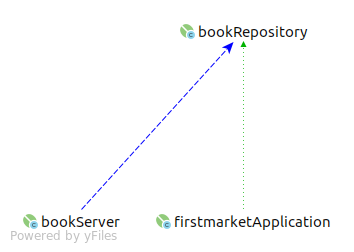
\includegraphics[width=0.6\textwidth]{di_bookRepository}
		\caption{Creación e inyección de dependencias en BookRepository}
		\label{fig:di_bookRepository}
	\end{figure}

	\begin{figure}[htb!]
		\centering
		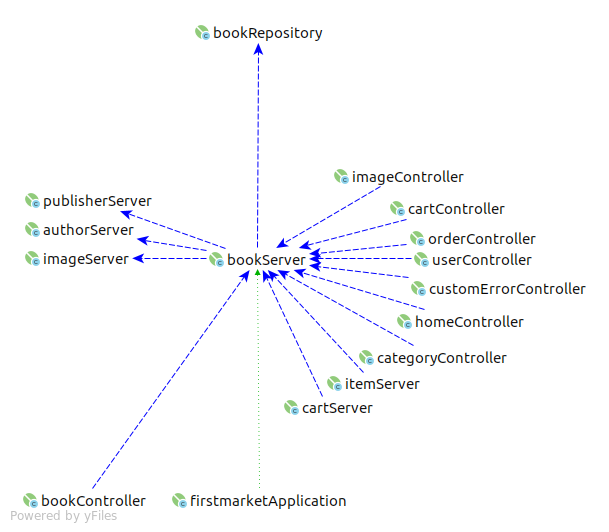
\includegraphics[width=\textwidth]{di_bookServer}
		\caption{Creación e inyección de dependencias en BookServer}
		\label{fig:di_bookServer}
	\end{figure}

	\begin{figure}[htb!]
		\centering
		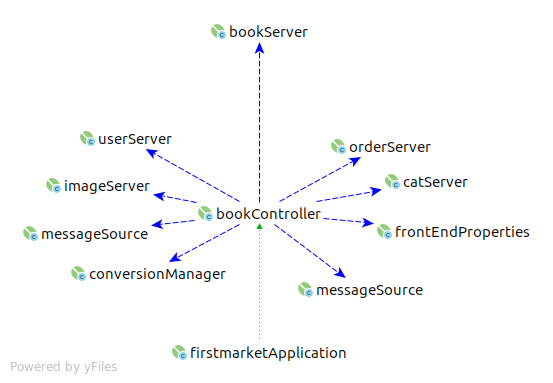
\includegraphics[width=\textwidth]{di_bookController}
		\caption{Creación e inyección de dependencias en BookContoller}
		\label{fig:di_bookController}
	\end{figure}
    
    \subsection{Capas funcionales} \label{sec:design_layer}
    Otro paso importante dado en la dirección de separar las responsabilidades es la división funcional del código en tres capas: web, negocio y persistencia. Estas capas están contenidas dentro del paquete \emph{core}, y están inspiradas en el patrón de diseño \emph{Fron Controller}, que es el que ordena, a su vez, la infraestructura web que proporciona Spring Framework (ver sección \ref{sec:spring}).
    
    \begin{figure}[htb!]
    	\centering
    	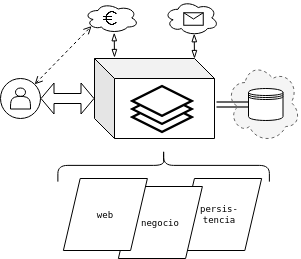
\includegraphics[width=0.75\textwidth,keepaspectratio]{desing_layer}
    	\caption{Modelo del sistema en capas funcionales}
    	\label{fig:desing_layer}
    \end{figure}
    
    La capa web se encarga de gestionar las peticiones HTTP encauzadas a través del \emph{DispatcherServler} y de resolver y generar el contenido HTML. A parte de toda la infraestructura que ofrece Spring Framework para esta tarea, se ha desarrollado una serie de \emph{controladores} (anotados con \emph{@Controller}), contenidos en el paquete \emph{core.controller} (ver figura \ref{fig:package_controller}), que sirven un conjunto de \emph{vistas}, contenidas en \emph{classpath: resources/templates}. Esta capa recibe el servicio de la capa de negocio.
    	
   	\begin{figure}[htb!]
   		\centering
   		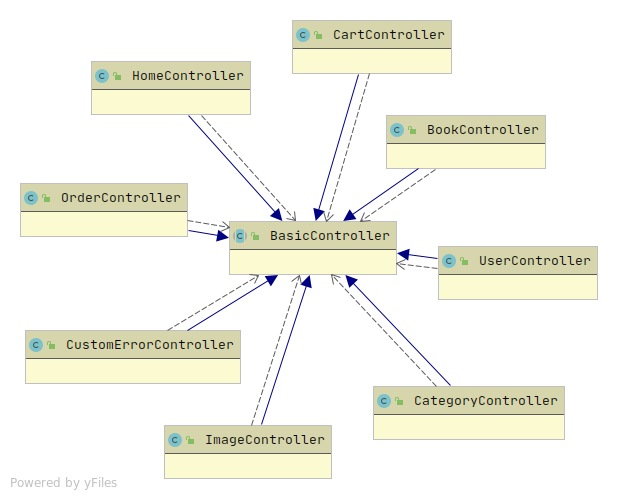
\includegraphics[width=0.7\textwidth,keepaspectratio]{package_controller}
   		\caption{Diagrama del paquete core.controller}
   		\label{fig:package_controller}
   	\end{figure}

   	\begin{figure}[htb!]
   		\centering
   		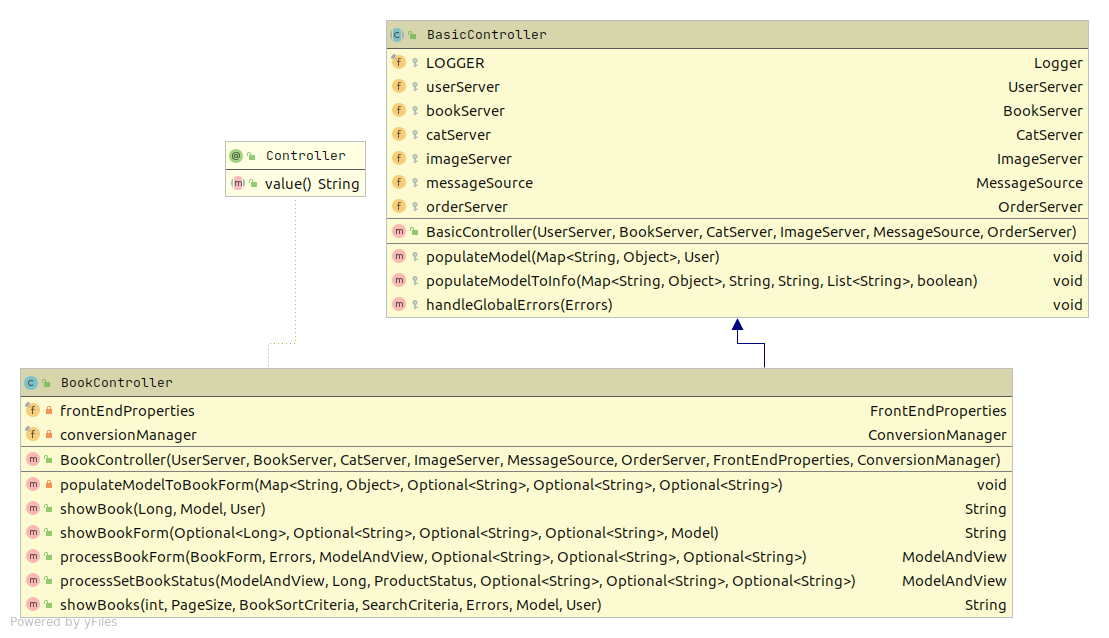
\includegraphics[width=\textwidth,keepaspectratio]{detail_bookController}
   		\caption{Detalle de la clase BookController}
   		\label{fig:detail_bookController}
   	\end{figure}
    	
   	En la capa de negocio reside la lógica (objetos anotados con \emph{@Service}) que modela el funcionamiento de una tienda de libros a través del código contenido en el paquete \emph{core.service} (ver figura \ref{fig:package_service}). Esta capa da servicio a la capa web y a sí misma, mientras que se apoya en el servicio que le ofrece la capa de persistencia.
    	
   	\begin{figure}[htb!]
		\centering
		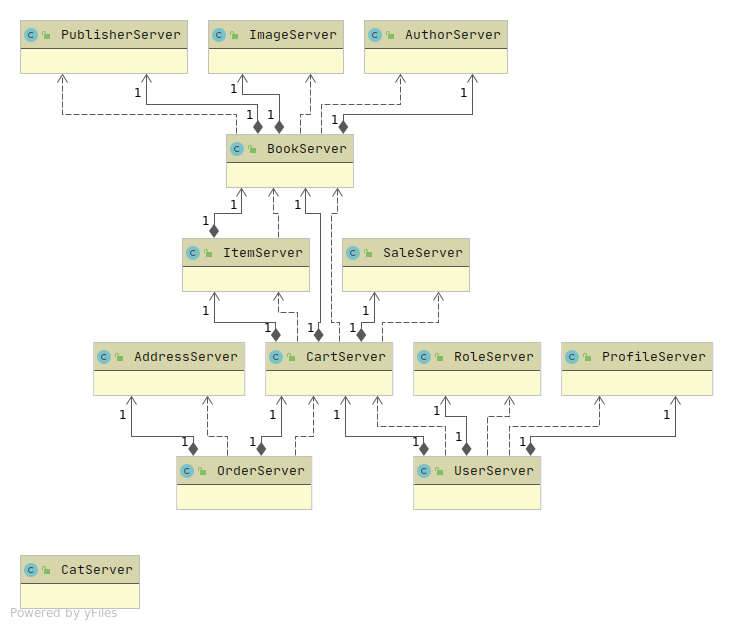
\includegraphics[width=\textwidth,keepaspectratio]{package_service}
		\caption{Diagrama del paquete core.service}
		\label{fig:package_service}
	\end{figure}

	\begin{figure}[htb!]
		\centering
		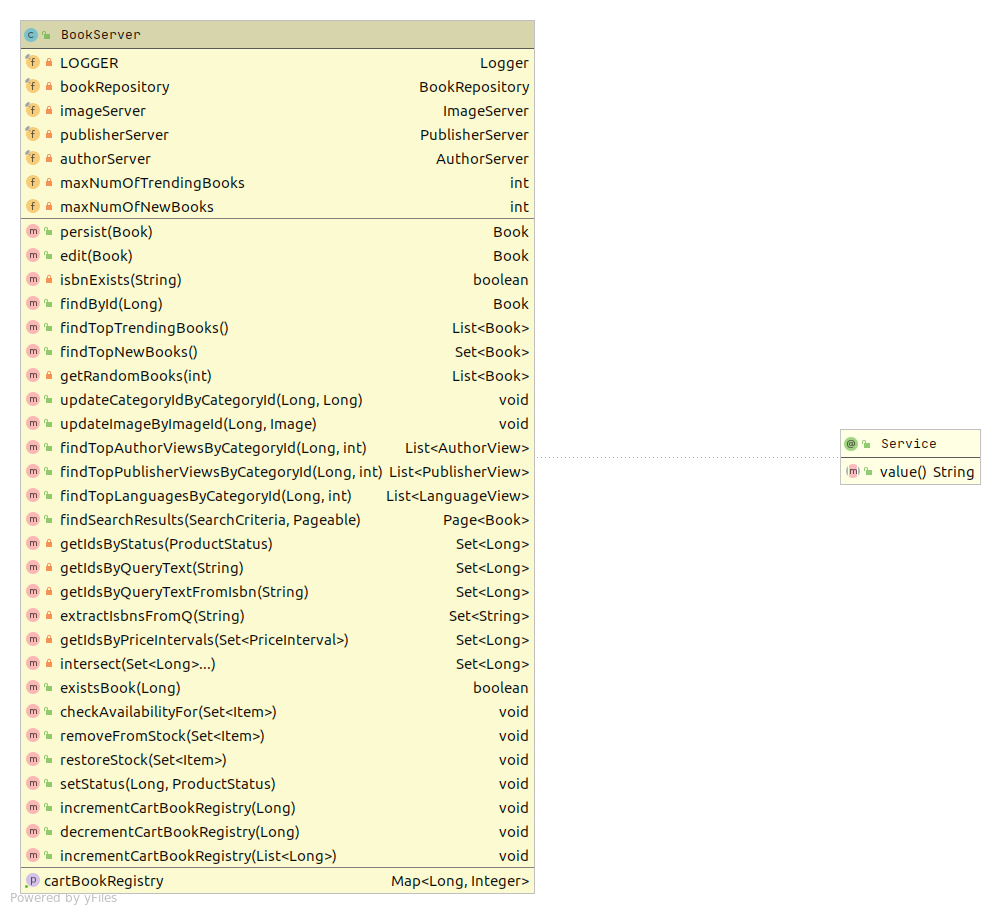
\includegraphics[width=\textwidth,keepaspectratio]{detail_bookServer}
		\caption{Detalle de la clase BookServer}
		\label{fig:detail_bookServer}
	\end{figure}

   	La capa de persistencia sigue el patrón de diseño \href{https://thorben-janssen.com/implementing-the-repository-pattern-with-jpa-and-hibernate/}{\emph{Repositorio}}. Así, toma el control de todos los aspectos relacionados con la solución concreta de almacenamiento y manipulación de los datos, desacoplando por completo esta funcionalidad de la lógica de negocio, a la cual sirve mediante un conjunto de interfaces (anotadas con \emph{@Repository}) definidas en \emph{core.data} (ver figura \ref{fig:package_data}).
    	
   	\begin{figure}[htb!]
   		\centering
   		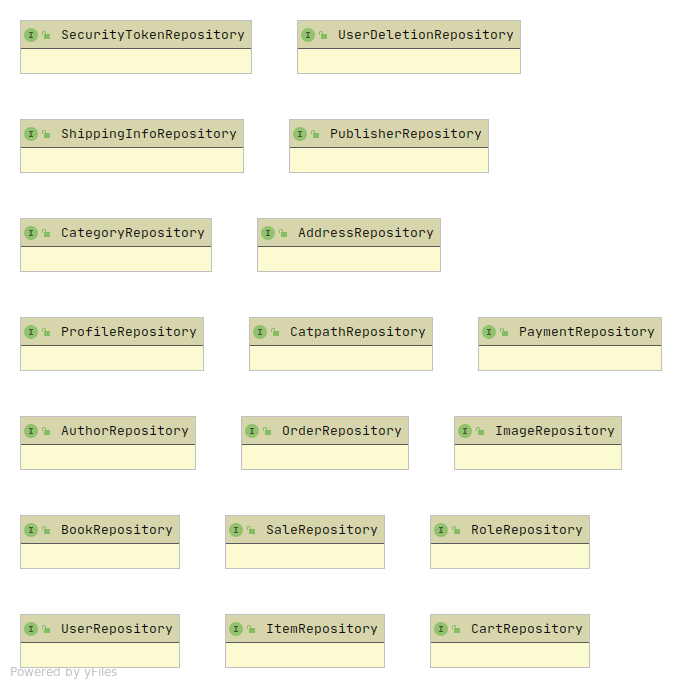
\includegraphics[width=\textwidth,keepaspectratio]{package_data}
   		\caption{Diagrama del paquete core.data}
   		\label{fig:package_data}
   	\end{figure}
   	
   	\begin{figure}[htb!]
   		\centering
   		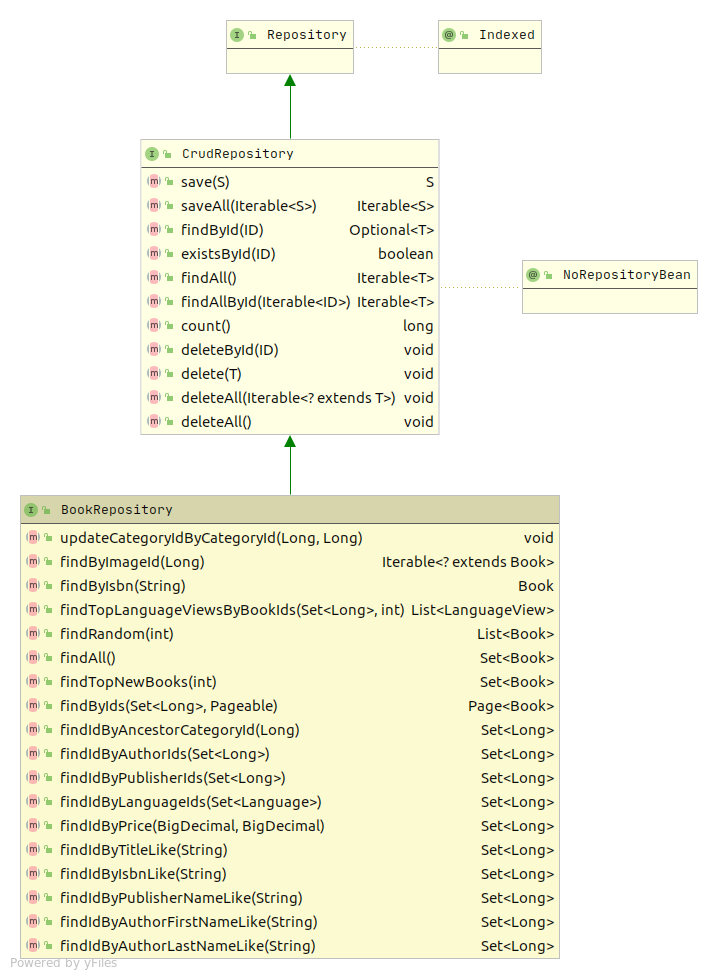
\includegraphics[width=\textwidth,keepaspectratio]{detail_bookRepository}
   		\caption{Detalle de la interfaz BookRepository}
   		\label{fig:detail_bookRepository}
   	\end{figure}
    	
    
    \section{Modelo de Datos}
    Para dar solución al problema presentado (la venta de libros online) se ha realizado un modelado de entidades del mundo real. Estas entidades se encuentran definidas en el paquete \emph{core.model}. En la figura \ref{fig:package_model} se muestra el diagrama de clases de este paquete. Este modelo encuentra una traducción directa en las entidades gestionadas en la base datos. En las figuras \ref{fig:er_simple_diagram} y \ref{fig:er_expanded_diagram} se ofrecen, respectivamente, los diagramas entidad relación sin y con las propiedades de los objetos visibles.
    
    \begin{figure}[htb!]
    	\centering
    	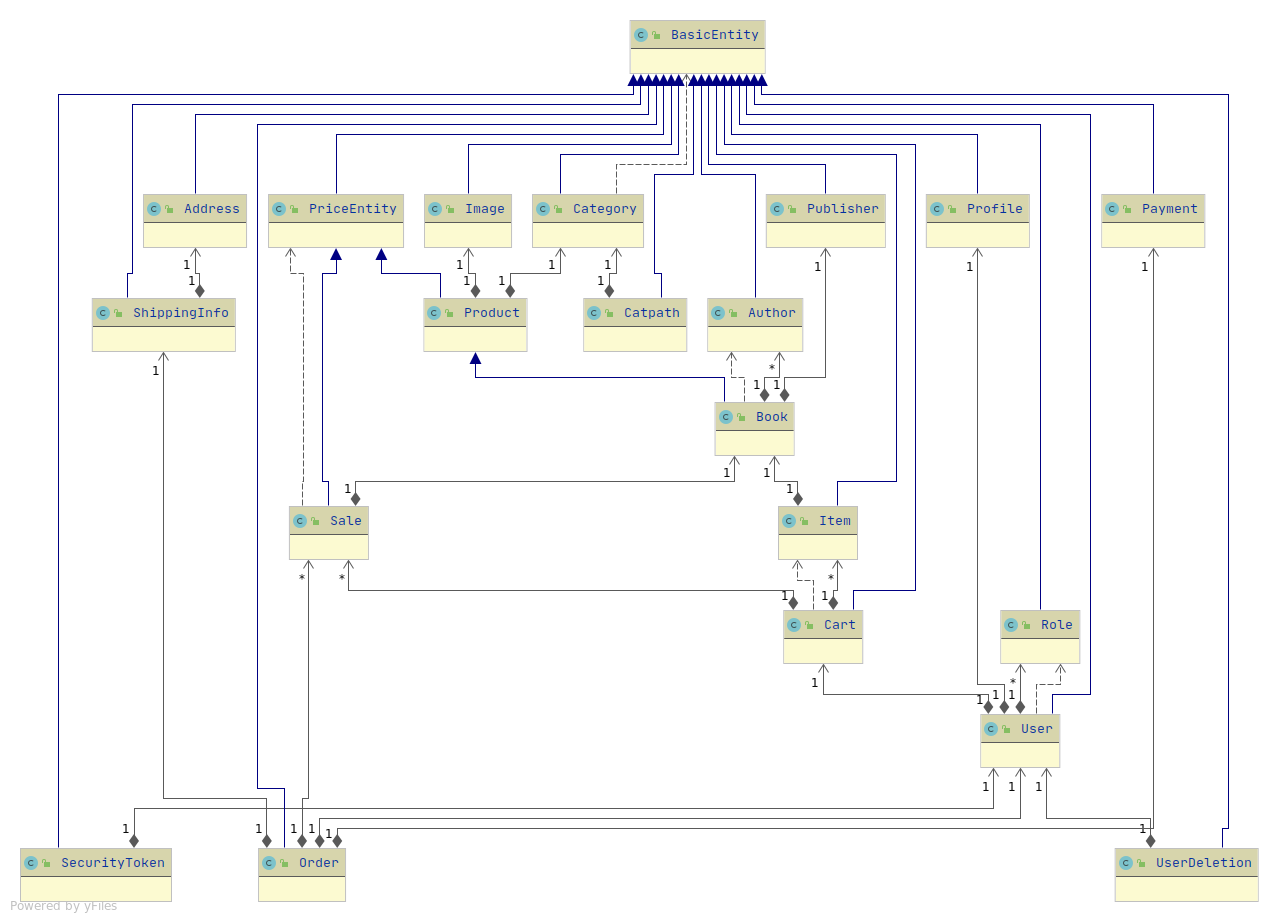
\includegraphics[height=\textwidth,angle=90,origin=c]{package_model}
    	\caption{Diagrama de clases del paquete core.model}
    	\label{fig:package_model}
    \end{figure}

	\begin{figure}[htb!]
		\centering
		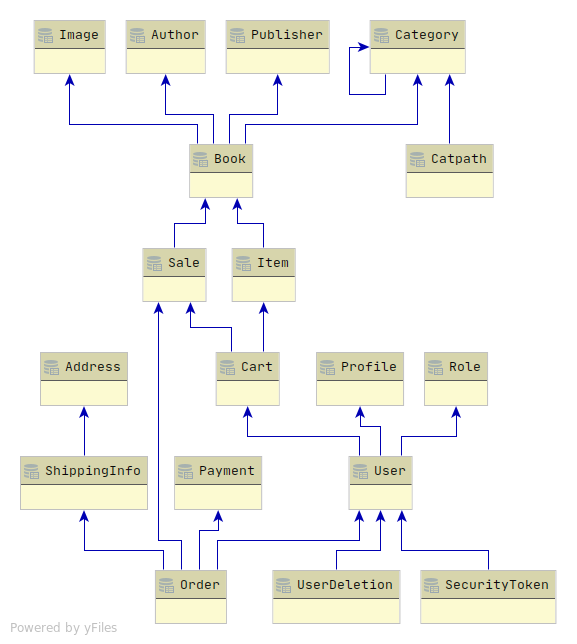
\includegraphics[width=\textwidth,keepaspectratio]{er_simple_diagram}
		\caption{Diagrama entidad-relación}
		\label{fig:er_simple_diagram}
	\end{figure}

	\begin{figure}[htb!]
		\centering
		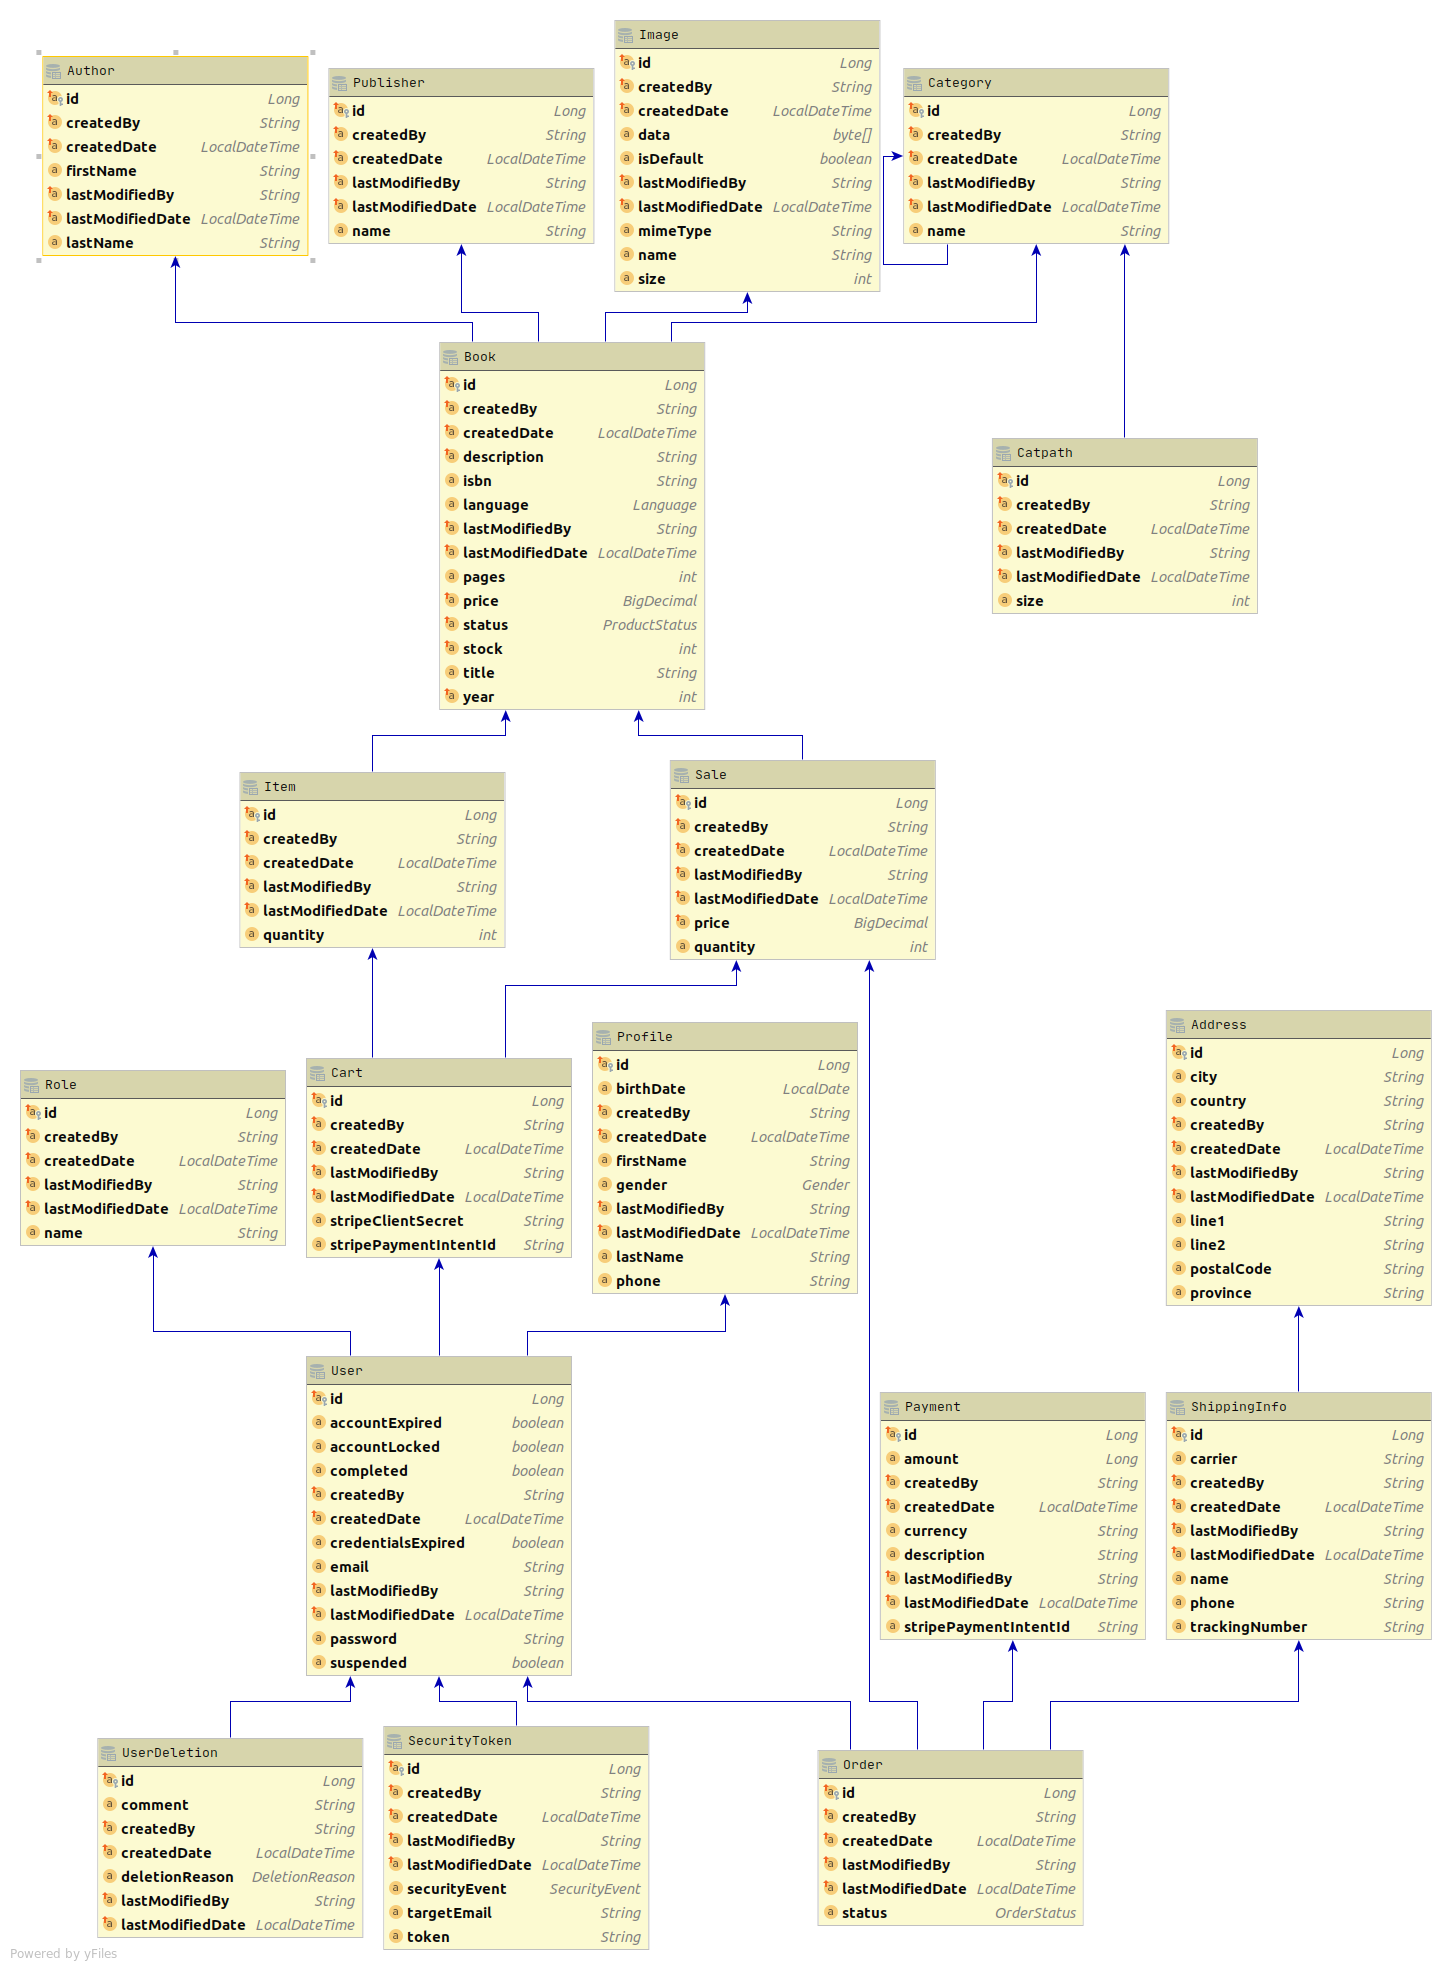
\includegraphics[width=\textwidth,keepaspectratio]{er_expanded_diagram}
		\caption{Diagrama entidad-relación expandido}
		\label{fig:er_expanded_diagram}
	\end{figure}